
%version 2: \usepackage{hyperref}


%%%%%%%%%%%%%%%%%%%%%%%%%%%%%%%%%%%%%%%%%%%%%%%%%%%%%%%%%%%%%%%%%%%%%%%%
%Para las ecuaciones siempre es Ec.(n).
%Para las figuras siempre es Fig.n, incluso en el caption de la figura. Tambien las Tablas
%Para las referencias es [n]
%%%%%%%%%%%%%%%%%%%%%%%%%%%%%%%%%%%%%%%%%%%%%%%%%%%%%%%%%%%%%%%%%%%%%%%%

\documentclass[
reprint,
%notitlepage,
%superscriptaddress,
%groupedaddress,
%unsortedaddress,
%runinaddress,
%frontmatterverbose, 
%preprint,
%showpacs,preprintnumbers,
%nofootinbib,
%nobibnotes,
%bibnotes,
%11 pt,
amsmath,
amssymb,
%aps,
%pra,
prb,
%rmp,
%tightenlines %esto hizo el milagro de sacar los espacios en blancos estocásticos (?)
%prstab,
%prstper,
%floatfix,\textbf{}
]{revtex4-1} %Instalar primero para usarlo. Paquete malo.

%\documentclass[onecolumn, aps, amsmath,amssymb ]{article}
\usepackage{lipsum}  
\usepackage{graphicx}% Include figure files
\usepackage{subfig}
\usepackage{braket}
\usepackage{comment} %comment large chunks of text
\usepackage{dcolumn}% Align table columns on decimal point
\usepackage{bm}% bold math
%\usepackage{hyperref}% add hypertext capabilities
\usepackage[mathlines]{lineno}% Enable numbering of text and display math
%\linenumbers\relax % Commence numbering lines
\usepackage{mathtools} %% Para el supraíndice

\usepackage[nice]{nicefrac}

%%%%%%%El Señor Español%%%%%%%%%%%%%%%%%%%%%%%%%%%
\usepackage[utf8]{inputenc} %acento
\usepackage[
spanish, %El lenguaje.
es-tabla, %La tabla y no cuadro.
activeacute, %El acento.
es-nodecimaldot %Punto y no coma con separador de números
]{babel}
\usepackage{microtype} %para hacerlo más bonito :33 como vos (?) 
%%%%%%%%%%%%%%%%%%%%%%%%%%%%%%%%%%%%%%%%%%%%%%%%%%%
%%%%%%%%% Para que las imágenes se queden dónde las quiero (?
\usepackage{float}
%%%%%%%%%%
\usepackage{enumitem}
\usepackage{hyperref} % Para usar \url

%%%%%%%%Cambia a Fig de Figure%%%%%%%%%%
\makeatletter
\renewcommand{\fnum@figure}{Fig. \thefigure} 
\makeatother
%%%%%%%%%%%%%%%%%%%%%%%%%%%%%%%%%%%%%%%%
\raggedbottom

\usepackage{multirow}
\begin{document}

\title{Práctica 2: Introducción a Keras}
\author{Evelyn~G.~Coronel}

\affiliation{Redes Neuronales y Aprendizaje Profundo para Visión Artificial\\ Instituto Balseiro\\}

\date[]{\lowercase{\today}} 

\maketitle

\section*{Ejercicio 1}

Considerando los valores de los inmuebles en Boston, se implementa un modelo simple de regresión lineal para predecir los precios, dadas las características de la propiedad. Este conjunto de datos es provisto por \verb|scikit| y las características que tienen los datos son, por ejemplo, índice de criminalidad en el barrio, edad media de los habitantes de la propiedad o los mismos son de clase baja o media para arriba.


Previo al modelo, los datos son preprocesados restando la media y normalizando por la desviación estándar. Luego se implementa una red con una función de activación lineal, con el uso de bias y la función de costo MSE. La pérdida de la red para los datos de entrenamiento y validación se muestra en la Fig.\,\ref{fig:ejer1_loss}, utilizando `SGD' con una tasa de aprendizaje del 0.001.


\begin{figure}[H]
    \begin{small}
        \begin{center}
            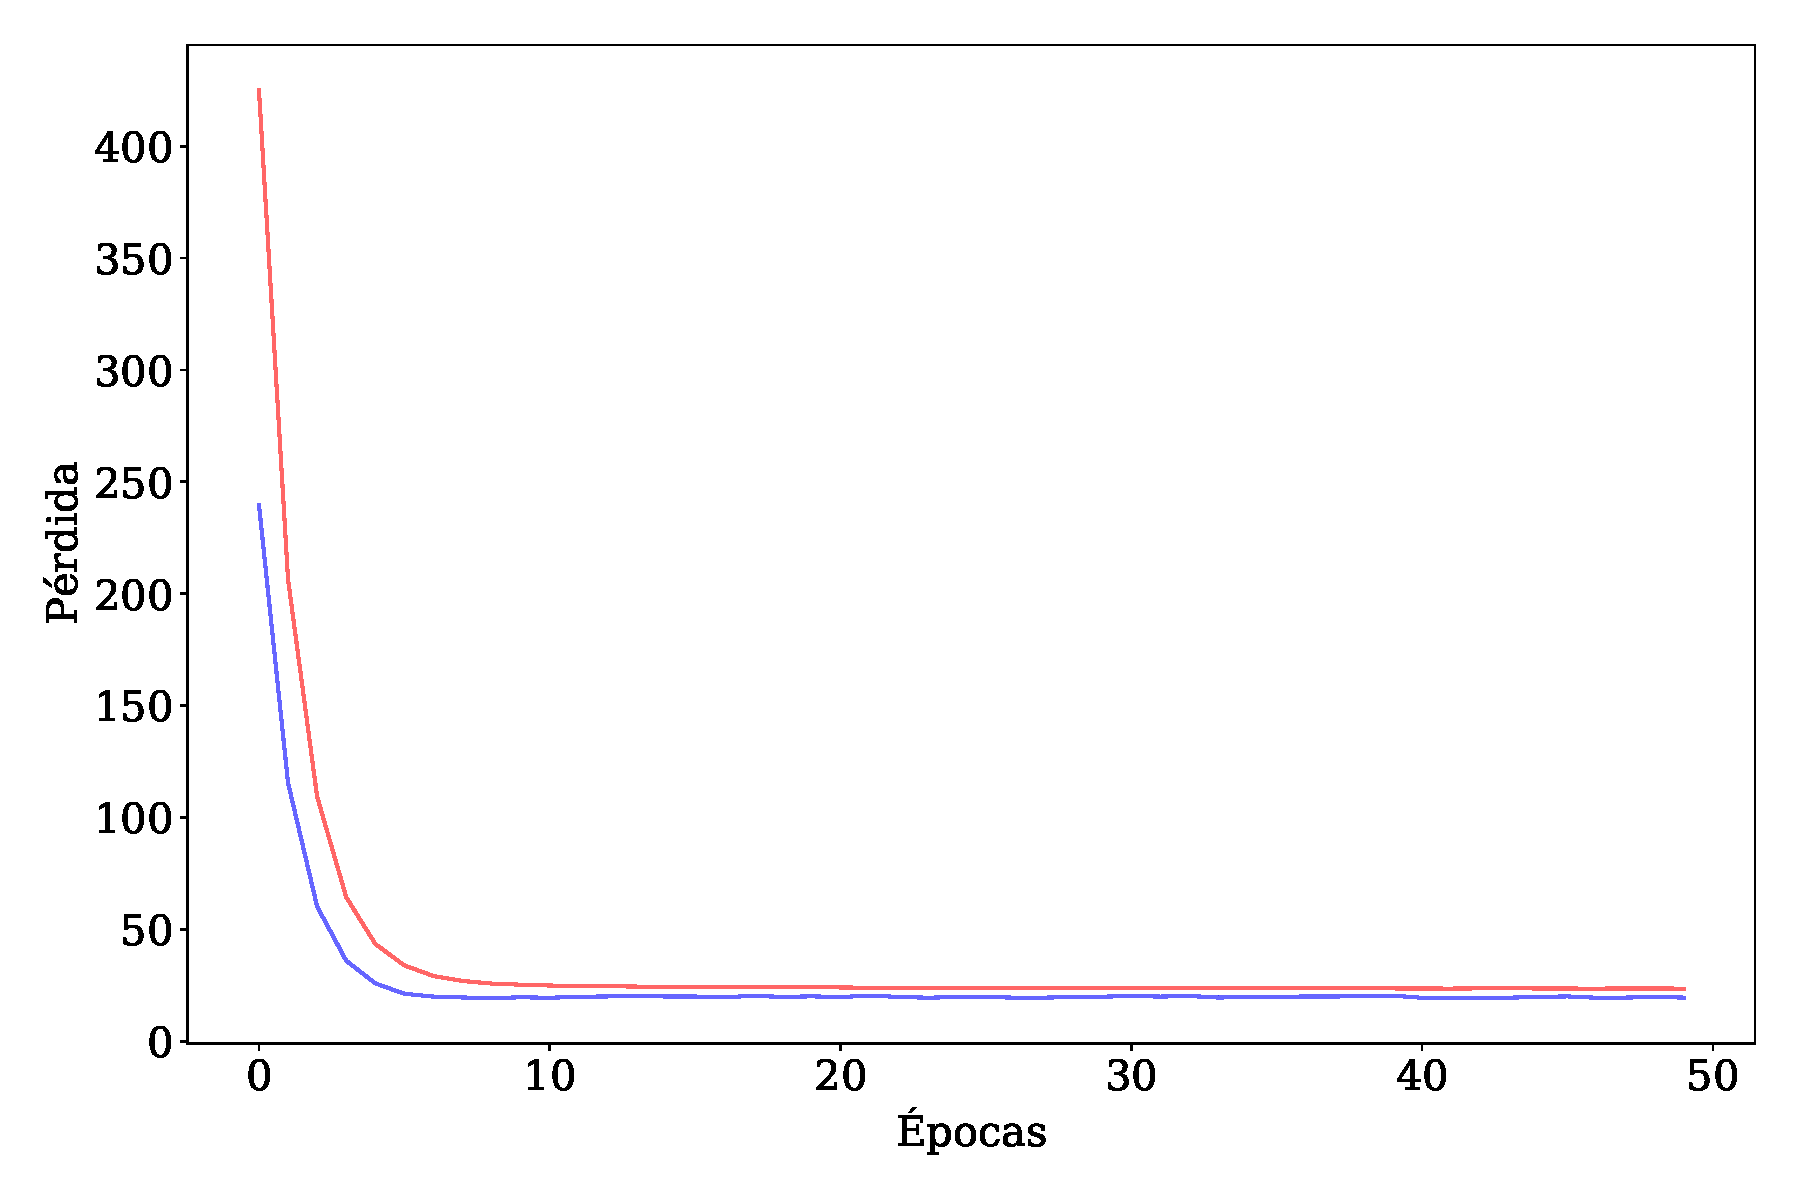
\includegraphics[width=0.5\textwidth]{Graphs/ejer1_loss.pdf}
        \end{center}
        \caption{Pérdida en función de las épocas para el ejercicio 1.}
        \label{fig:ejer1_loss}
    \end{small}
\end{figure}

Para dimensionar la efectividad de la red, en la Fig.\,\ref{fig:ejer1_comparacion} se muestra una comparación entre los precios reales de los inmuebles con los precios predichos por la red para los datos de validación. La línea de referencia marca los puntos donde los precios reales y predichos son iguales, se observa que la red tiene una dispersión con respecto a la referencia.

\begin{figure}[H]
    \begin{small}
        \begin{center}
            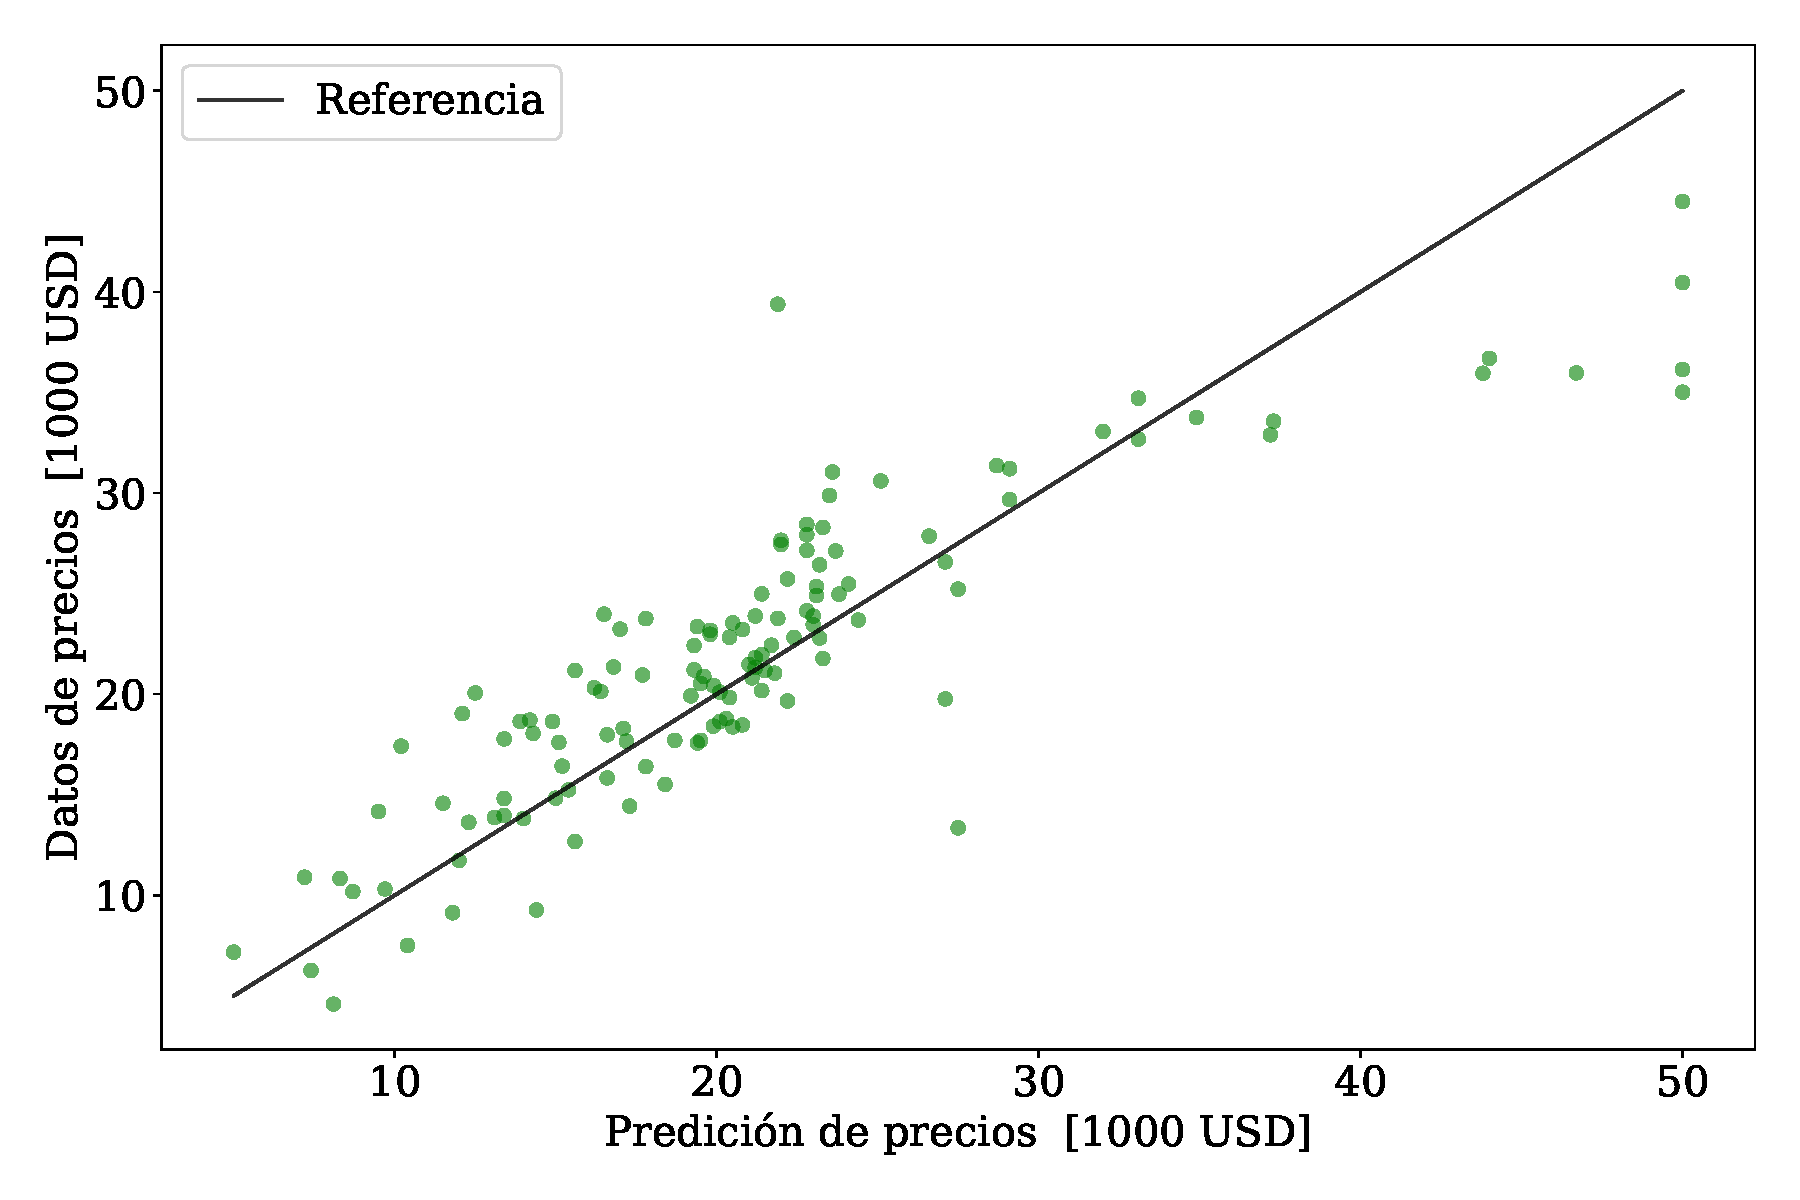
\includegraphics[width=0.5\textwidth]{Graphs/ejer1_versus.pdf}
        \end{center}
        \caption{Comparación de precios reales y predichos en los datos de validación}
        \label{fig:ejer1_comparacion}
    \end{small}
\end{figure}

Otra forma de dimensionar la efectividad de la red, es comprobar si la red capta la correlación entre una característica y el precio del inmueble. Por ejemplo, en el Fig.\,\ref{fig:ejer1_low_income} se muestran el precio de los inmuebles en función del porcentaje de personas en la clase baja, los datos en Boston dicen que los inmuebles en las zonas más  pobres tienden a tener un menor precio, esta correlación también se ve reflejado en los datos predichos por la red.

\begin{figure}[H]
    \begin{small}
        \begin{center}
            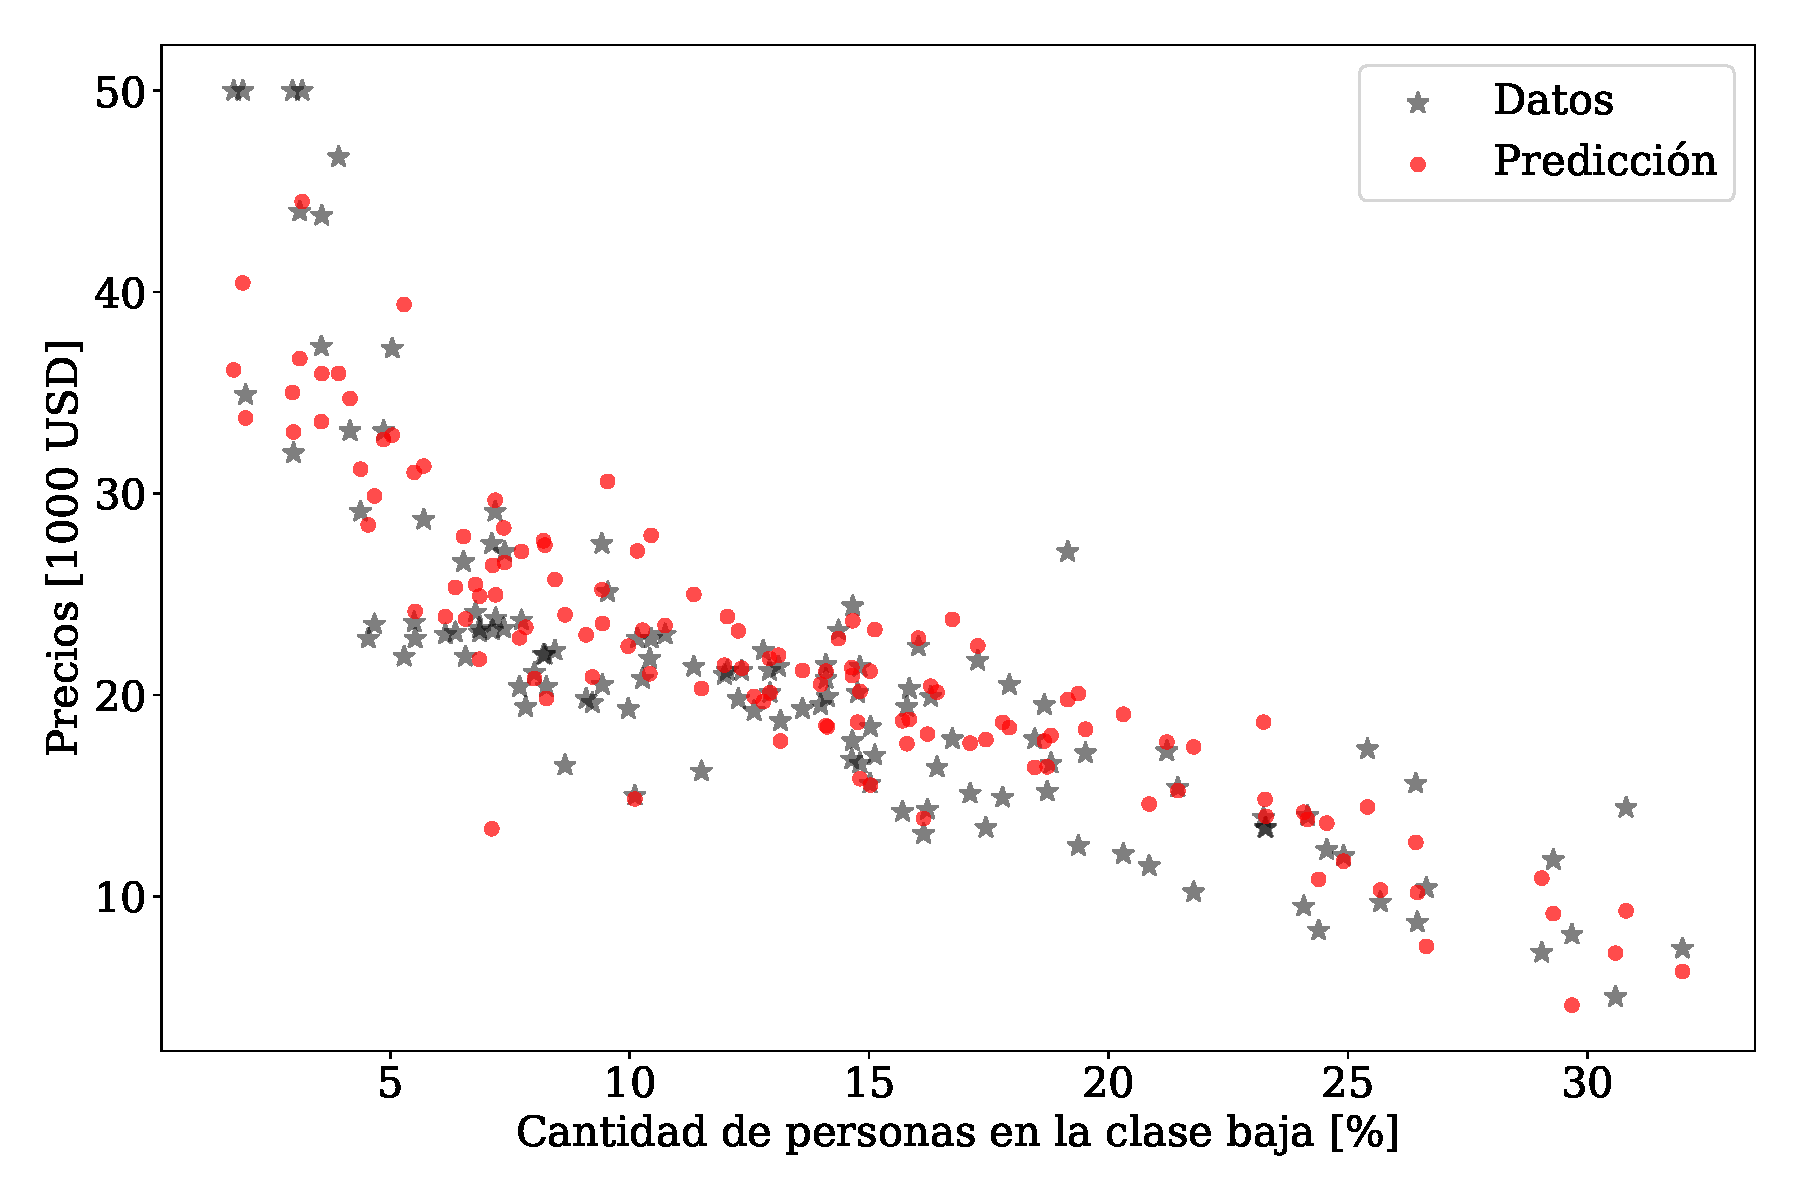
\includegraphics[width=0.5\textwidth]{Graphs/ejer1_low_income.pdf}
        \end{center}
        \caption{Precio reales y predichos de los inmuebles en función del porcentaje de personas en la clase baja}
        \label{fig:ejer1_low_income}
    \end{small}
\end{figure}


\section*{Ejercicio 7}




\end{document}